\section{Návrh a analýza finální geometrie} \label{sec:finalni-geometrie}
    \subsection{Návrh konstrukčních úprav}
        Změny v rámci konstrukce sondy se týkaly zejména rozměrů trubic a odvětrání čidla\,A. Vzhledem k malému přínosu přidání difuzoru nebo kavit nebyly tyto konstrukční úpravy ve finální verzi sondy implementovány. Zachována byla trubice tvořící tělo sondy (rozměr $4 \times 0.4 \Unit{mm}$) a těsnění na koncích teplotních čidel. Čelo snímače B bylo posunuto na stejnou úroveň, jako čelo čidla\,A. 
        
        Stínící trubice čidla A byla zvětšena na rozměr $5 \times 0.5 \Unit{mm}$ a odvětrání bylo posunuto na $18 \Unit{mm}$ od čela stínění. Odvětrávací otvory byly zmenšeny na průměr $0.5 \Unit{mm}$ a byl zvýšen jejich počet ze $2$ na $4$, rozmístěny byly rovnoměrně po obvodu stínění.

        Čidlo B bylo, jako v Kapitolách \ref{sec:sonda-se-stinenim-B} a \ref{sec:sonda-s-rozsirenym-stinenim-B}, opatřeno stíněním, v tomto případě tvořeném trubicí o rozměrech $9 \times 0.5 \Unit{mm}$, které bylo na koncích společně s trubicí uchycující čidlo B opatřeno zkosením $5^o$. Detailní rozměry modelu jsou uvedeny v\,Příloze \ref{fig:sonda-final-vykres}.

        Potřebný měricí prostor se zvětšil z rozměru $37.5 \times 9 \times 4$ na $31 \times 14 \times 9$ ($x \times y \times z$), viz Obrázek \ref{fig:sonda-final-porovnani}.

        \begin{figure}[ht!]
            \centering
            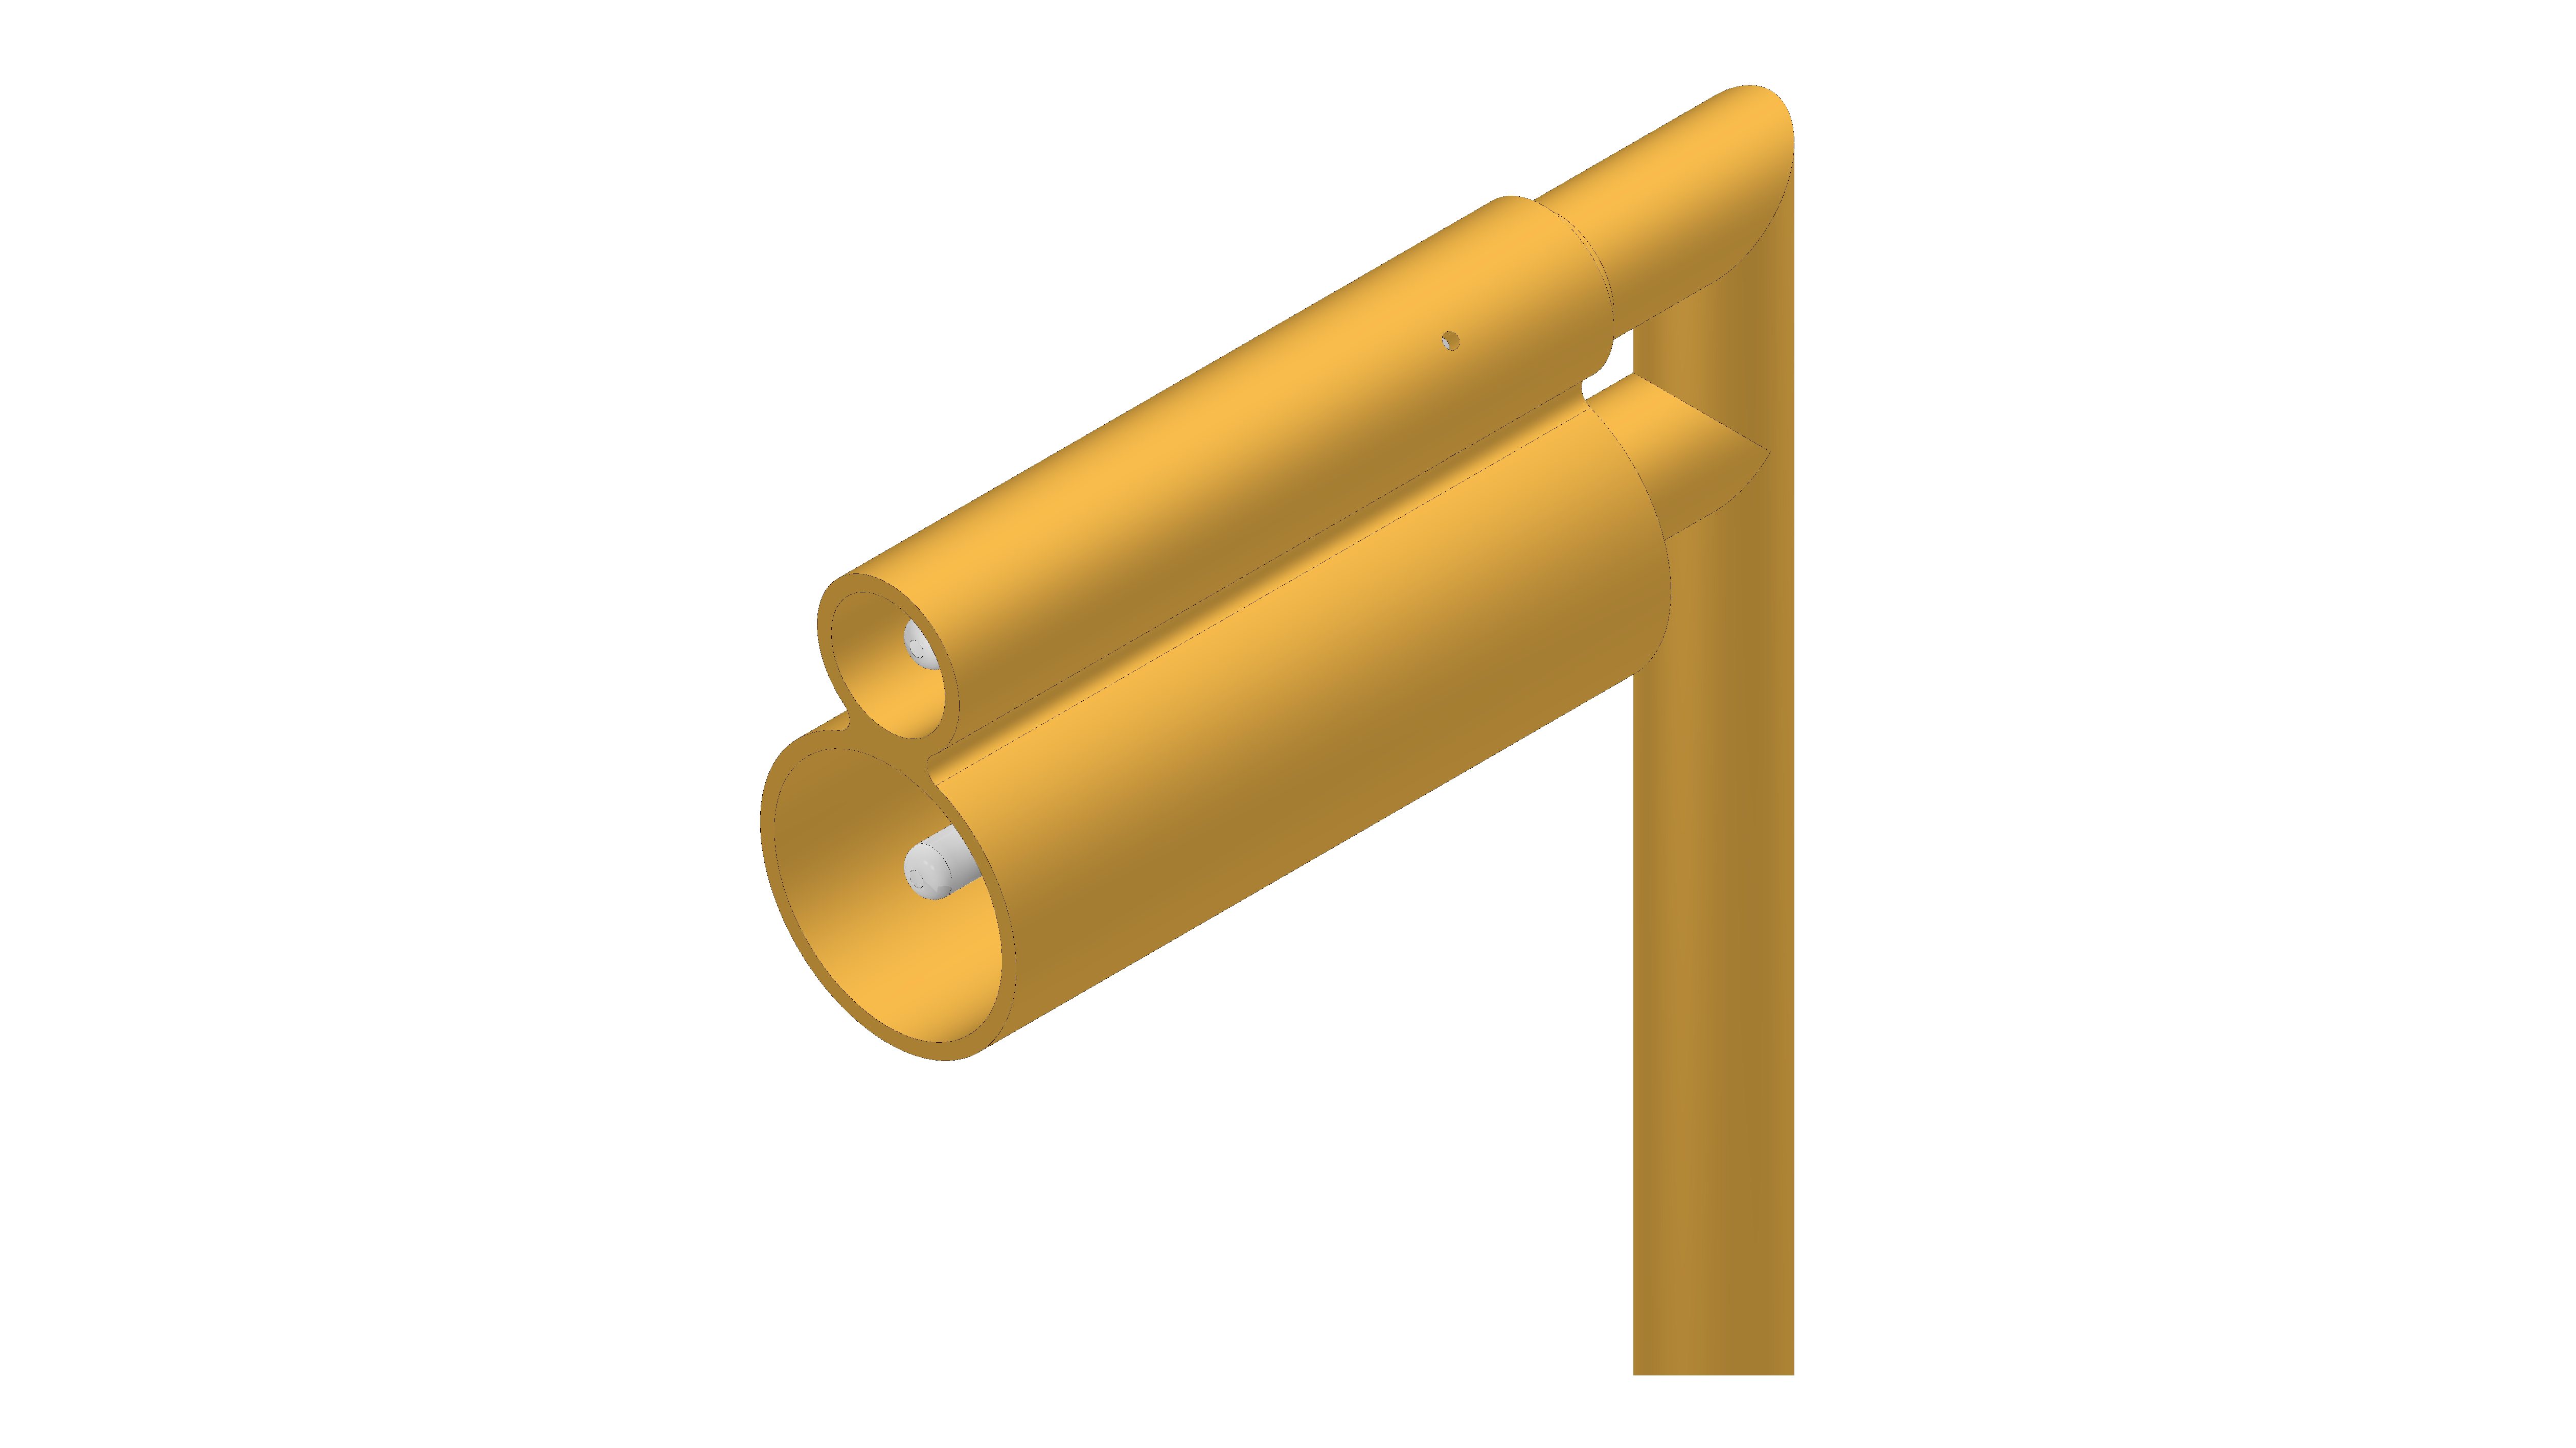
\includegraphics[width=\textwidth]{500_FINAL/sonda_final.png}
            \caption{Finální model DRTA sondy.}
            \label{fig:sonda-final}
        \end{figure}

        

        \begin{figure}[ht!]
            \centering
            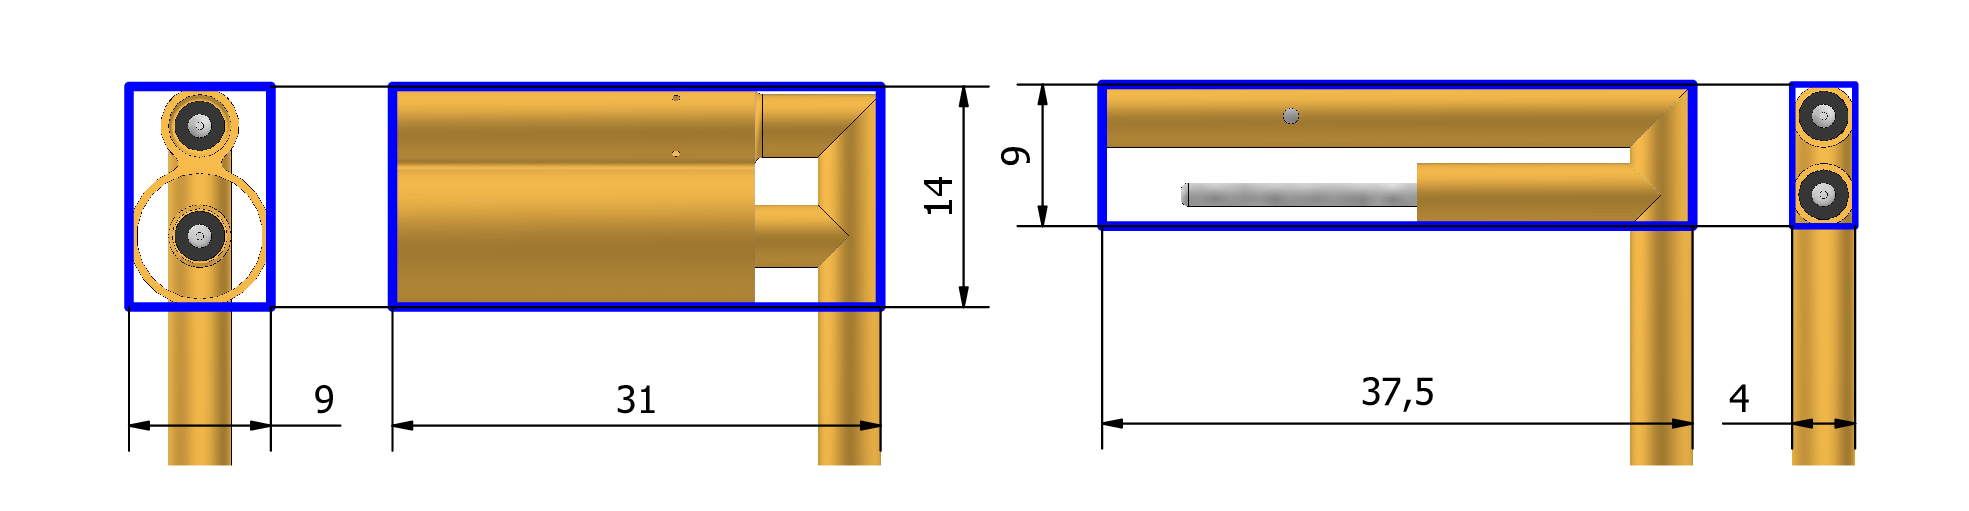
\includegraphics[width=\textwidth]{500_FINAL/porovnani_v01_final.png}
            \caption{Porovnání rozměrů finální (vlevo) a původní (vpravo) verze sondy.}
            \label{fig:sonda-final-porovnani}
        \end{figure}
        
    \subsection{CFD analýza}
        Chování restitučních faktorů bylo analyzováno stejným postupem, jako v Kapitolách \ref{sec:sonda-bez-stineni-B} a \ref{sec:sonda-s-rozsirenym-stinenim-B} – byla zkoumána jejich závislost na rychlosti proudění ($100 \div 325 \Unit{\frac{m}{s}}$ ) a\,na natočení v rovině symetrie a kolmo na ní (v rozmezí $\pm 15^o$). Nakonec byl zkoumán vliv materiálu trubice, kde byla mosaz nahrazena ocelí a poté polykarbonátem.
        \subsubsection{Chování při různých rychlostech proudění}
            Přidané stínění k čidlu B zajistilo částečné vyrovnání průběhu rozdílu restitučních faktorů, což je nejvíce patrné pro rychlosti proudění do $225 \Unit{\frac{m}{s}}$, viz Obrázek \ref{fig:sonda-final-rychlosti}. Při dalším zvyšování Machova čísla docházelo k poklesu rozdílu až na $92 \Unit{\%}$ hodnoty odpovídající rychlosti $250 \Unit{\frac{m}{s}}$, která byla rovna $0.1232$. 
            \begin{figure}[ht!]
                \centering
                \includegraphics*[width=\textwidth]{500_FINAL/final_rychlosti.eps}
                \caption{Závislost restitučních faktorů upravené sondy na rychlosti proudění.}
                \label{fig:sonda-final-rychlosti}
            \end{figure}

            Restituční faktor čidla A vzrostl v průměru o přibližně $2.03 \Unit{\%}$, nárůst u čidla B byl $1.76 \Unit{\%}$ pro rychlost $250 \Unit{\frac{m}{s}}$ a $2.54 \Unit{\%}$ pro rychlost $325 \Unit{\frac{m}{s}}$. Při nejnižší zkoumané rychlosti restituční faktor poklesl o $1.33 \Unit{\%}$, došlo tedy ke zlepšení jeho výsledného průběhu (přiblížení k \uv{rovnoběžným} průběhům), což se promítlo do již zmíněného vyrovnání rozdílu restitučních faktorů.

            \begin{figure}[ht!]
                \centering
                \begin{subfigure}{0.45\textwidth}
                    \centering
                    \captionsetup{width=.9\linewidth}
                    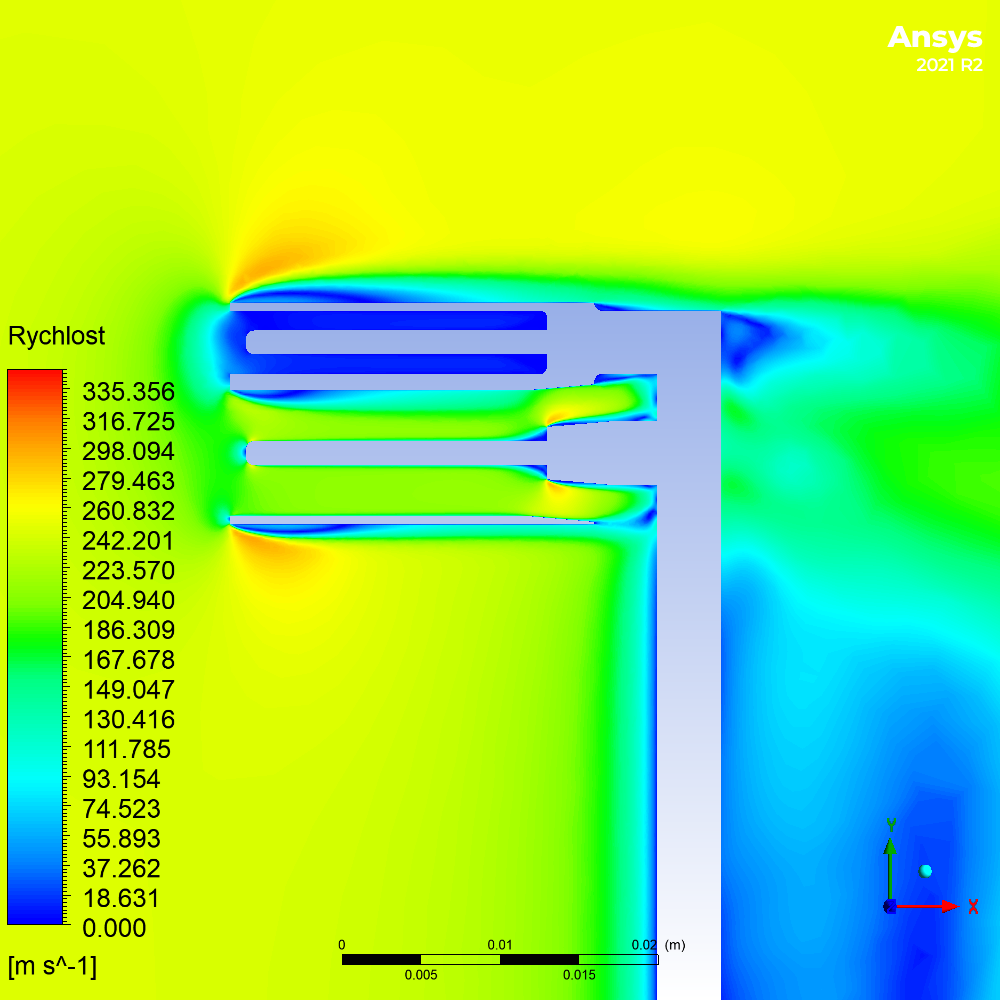
\includegraphics[width=\textwidth]{500_FINAL/SIM_Final_XY0_rychlost.png}
                    \caption{Rychlostní pole.}
                \end{subfigure}
                \begin{subfigure}{0.45\textwidth}
                    \centering
                    \captionsetup{width=.9\linewidth}
                    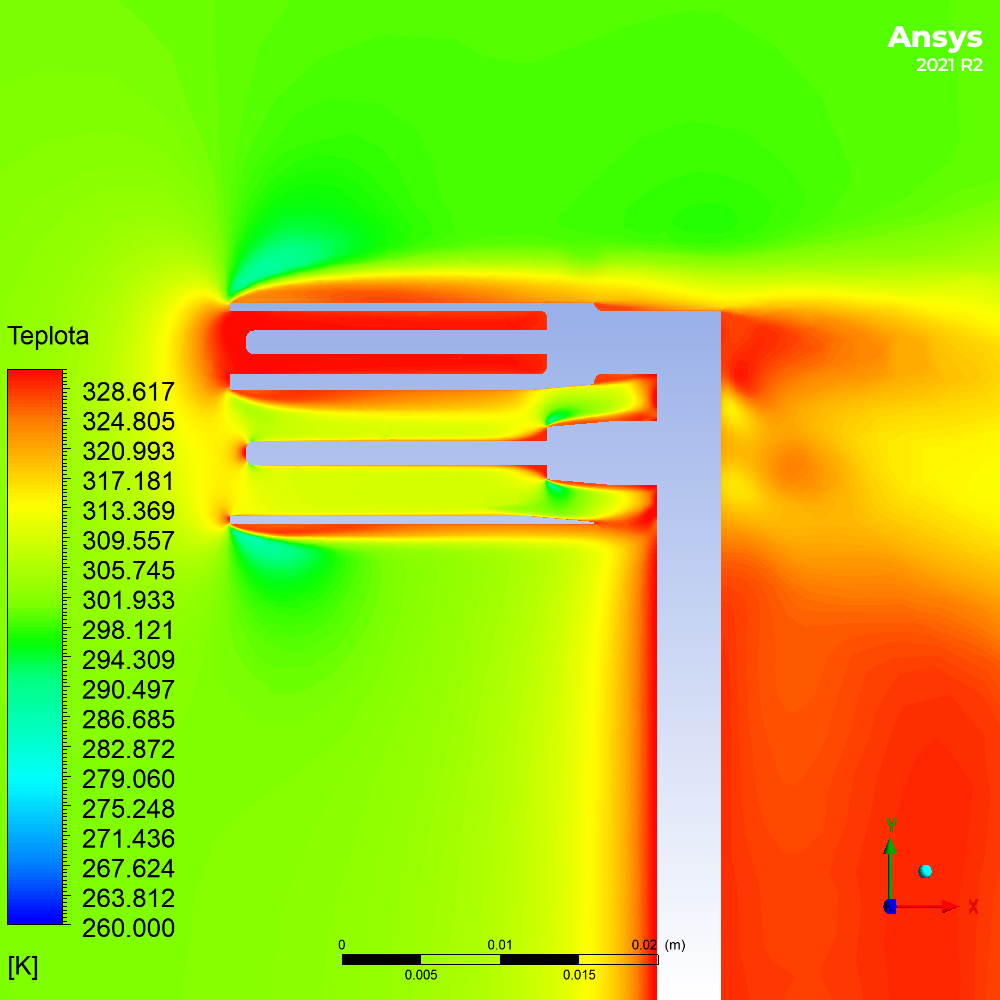
\includegraphics[width=\textwidth]{500_FINAL/SIM_Final_XY0_teplota.png}
                    \caption{Teplotní pole.}
                \end{subfigure}
                \caption{Vizualizace vypočtených dat pro upravenou sondu v rovině symetrie pro rychlost proudění $250 \Unit{\frac{m}{s}}$.}
                \label{fig:sonda-final-vizualizace}
            \end{figure}

        \newpage
        \subsubsection{Směrová citlivost v rovině symetrie}
            Oproti původní geometrii sondy nedocházelo k tak výraznému narušení proudění v\,okolí čidla B (viz Obrázek \ref{fig:sonda-final-symetrie}) – původní odchylka $45.9 \Unit{\%}$ rozdílu restitučních faktorů při vychýlení $-15^o$ se zmenšila na $9.85 \Unit{\%}$. Došlo rovněž k vyrovnání průběhu rozdílu při natáčení sondy opačným směrem.
            \begin{figure}[ht!]
                \centering
                \includegraphics*[width=\textwidth]{500_FINAL/final_XY.eps}
                \caption{Závislost restitučních faktorů upravené sondy na natočení v rovině symetrie.}
                \label{fig:sonda-final-symetrie}
            \end{figure}
        \newpage

        \subsubsection{Směrová citlivost kolmo na rovinu symetrie}
            Změna restitučních faktorů při natáčení sondy v rovině $XZ$ zůstala podobná, jako v případě původní geometrie (došlo pouze ke změně jejich velikosti, viz Obrázek \ref{fig:sonda-final-kolma-rovina}).
            \begin{figure}[ht!]
                \centering
                \includegraphics*[width=\textwidth]{500_FINAL/final_XZ.eps}
                \caption{Závislost restitučních faktorů upravené sondy na natočení kolmo na rovinu symetrie.}
                \label{fig:sonda-final-kolma-rovina}
            \end{figure}

        \newpage
        \subsection{Zhodnocení}

            Vybrané konstrukční úpravy se ukázaly jako prospěšné zejména v oblasti směrové citlivosti sondy. Pro rychlost proudění $250 \Unit{\frac{m}{s}}$ bez natočení sondy byl rozdíl restitučních faktorů roven $0.1232$, nicméně tato hodnota se neukázala jako konstantní. Relativní odchylka rozdílu restitučních faktorů se v rámci vypočtených dat pohybovala v rozmezí $\pm10 \Unit{\%}$, viz Obrázek \ref{fig:sonda-final-rozdil-restitucnich-faktoru}. Zde je patrné, že největší odchylka nastala při rychlostech nad $275 \Unit{\frac{m}{s}}$ a při natočeních v rovině symetrie menších, než $-10^o$. Ostatní hodnoty se nacházely v pásmu $\pm5\%$ odchylky.

            \begin{figure}[ht!]
                \centering
                \includegraphics*[width=\textwidth]{500_FINAL/final_rozdil_restitucnich_faktoru.eps}
                \caption{Porovnání závislostí rozdílu restitučních faktorů s vyznačením $2.5\%$ ,$5\%$ a $10\%$\,odchylky od hodnoty v nevychýleném stavu a při rychlosti proudění $250 \Unit{\frac{m}{s}}$.}
                \label{fig:sonda-final-rozdil-restitucnich-faktoru}
            \end{figure}

            

            S využitím vztahu pro určení rychlosti proudění pomocí DRTA sondy (viz \linebreak Kapitola \ref{sec:DRTA-princip}) byla stanovena závislost mezi chybou měření $\varepsilon _u$ a chybou uvažování konstantního rozdílu restitučních faktorů $\varepsilon _f$ (viz odvození v Příloze \ref{sec:odvozeni-chyby}):
            \begin{equation} \label{eq:chyba-mereni}
                \varepsilon _u = 1 - \sqrt{\frac{1}{1 + \varepsilon _f}}
            \end{equation}
            Aplikací tohoto vztahu bylo získáno rozložení chyb měření pro jednotlivé počítané případy, viz Obrázek \ref{fig:sonda-final-chyba-mereni}. Zde je patrné, že zatímco se relativní odchylka většiny rozdílů restitučních faktorů pohybovala v pásmu $\pm5 \Unit{\%}$, tak vzhledem k nelinearitě závislosti byla výsledná chyba měření ve většině případů v rozmezí $\pm2.5 \Unit{\%}$. 

            \begin{figure}[ht!]
                \centering
                \includegraphics*[width=\textwidth]{500_FINAL/final_chyba_mereni.eps}
                \caption{Rozložení chyb měření rychlosti při uvažování konstantního rozdílu restitučních faktorů.}
                \label{fig:sonda-final-chyba-mereni}
            \end{figure}

        \newpage
        \subsection{Volba materiálu trubice}
            Vedle konstrukčních úprav sondy byla zkoumána také možnost změny materiálu trubice. Použitá mosaz má příznivé vlastnosti zejména ohledně konstrukčních možností – dobře se zpracovává a letuje, což v minulosti umožnilo výrobu prvního prototypu sondy pro experimentální testování. Při uvažování jejích fyzikálních vlastností se však nabízely i jiné materiály, které by v tomto ohledu mohly fungovat lépe. Mosaz vede dobře teplo, což mohlo ovlivnit zejména restituční faktor čidla A vlivem úniku tepla stíněním.

            Alternativní materiály byly zvoleny dva: ocel, jakožto dobře dostupná náhrada mosazi, a následně polykarbonát (PC). Použití PC by znamenalo možnost využití 3D tisku při konstrukci sondy pro experimentální testování, což by poskytlo prostor složitějším konstrukčním úpravám. Použité vlastnosti materiálů trubice jsou popsány v Tabulce \ref{tab:final-materialy}. Obě alternativy byly voleny i s přihlédnutím k jejich mechanickým vlastnostem, kdy zejména u PC je klíčová jeho dobrá pevnost i teplotní odolnost až \linebreak do $145 \Unit{^oC}$ \cite{Morgan1976}.

            \begin{table}[ht!]
                \centering
                \caption{Zkoumané materiály trubice.}
                \resizebox{\textwidth}{!}{%
                \begin{tabular}{l|l|l|l}
                                 & Hustota $\unit{\frac{kg}{m^3}}$ & Měrná tepelná kapacita $\unit{\frac{J}{kg \cdot K}}$ & Tepelná vodivost $\unit{\frac{W}{m \cdot K}}$ \\ \hline
                    Mosaz        & 8730                            & 400                                                  & 96                                            \\ \hline
                    Ocel         & 7700                            & 466                                                  & 45                                            \\ \hline
                    Polykarbonát & 1200                            & 1250                                                 & 0.2                                          
                \end{tabular}%
                }
                \label{tab:final-materialy}
            \end{table}

            \newpage

            Výsledky analýzy vlivu materiálu trubice jsou reprezentovány Obrázkem \ref{fig:sonda-final-materialy}. Testováno bylo chování restitučních faktorů pro celkem čtyři rychlosti proudění. Největší rozdíl je patrný u čidla A, kde došlo k nárůstu o $0.29 \Unit{\%}$ pro ocel a $0.99 \Unit{\%}$ pro polykarbonát. V případě čidla B nedošlo k žádným výrazným změnám, což odpovídá předpokladům. Výsledný rozdíl restitučních faktorů se zvýšil o $1.74 \Unit{\%}$ při použití oceli a o $6.29 \Unit{\%}$ při použití polykarbonátu.

            \begin{figure}[ht!]
                \centering
                \includegraphics*[width=\textwidth]{500_FINAL/final_material.eps}
                \caption{Vliv volby materiálu trubice na velikost restitučních faktorů.}
                \label{fig:sonda-final-materialy}
            \end{figure}


        
        